\subsection{The tensor product of extensions}

PROPOSITION 1. --- Let \(\Omega\) be an extension of a field \(K\) and let \(L, M\) be two subextensions of \(\Omega\) which are algebraically disjoint over \(K\) . Suppose that the relative separable algebraic closure of \(K\) in \(L\) is equal to \(K^1\) . Let \(\varphi\) be the K-algebra homomorphism of \(L \otimes_K M\) into \(\Omega\) mapping \(x \otimes y\) to \(xy\) for \(x \in L\) , \(y \in M\) , and let \(\mathfrak{p}\) be the kernel of \(\varphi\) . Then \(\mathfrak{p}\) is the set of nilpotent elements of \(L \otimes_K M\) and this is the smallest prime ideal of \(L \otimes_K M\) .

On replacing \(\Omega\) by an algebraic closure if necessary, we may suppose \(\Omega\) algebraically closed. Let B be a transcendence basis of M over K, N the relative algebraic closure of \(\mathrm{K}(\mathrm{B})\) in \(\Omega\) and \(\mathrm{N}_{s}\) (resp. \(N_{r}\) ) the set of elements of N which are separable (resp. p-radical) over \(\mathrm{K}(\mathrm{B})\) . We remark that M is algebraic over \(\mathrm{K}(\mathrm{B})\) , so that N is the relative algebraic closure of M in \(\Omega\) .

\pandocbounded{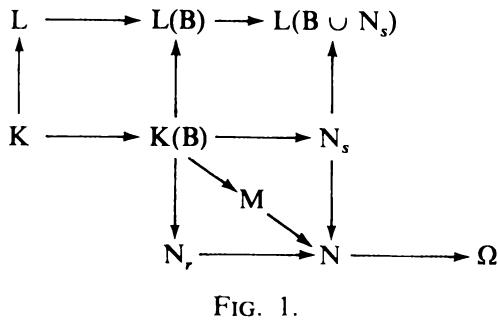
\includegraphics[keepaspectratio]{images/part002_5eeda79f.jpg}}

Let us define the following chain of homomorphisms :

\[
\begin{array}{r l} & {\mathrm{L} \otimes_ {\mathrm{K}} \mathrm{M} \xrightarrow {\alpha} \mathrm{L} \otimes_ {\mathrm{K}} \mathrm{N} \xrightarrow {\beta} (\mathrm{L} \otimes_ {\mathrm{K}} \mathrm{K} (\mathrm{B})) \otimes_ {\mathrm{K} (\mathrm{B})} \mathrm{N} \xrightarrow {\gamma} \mathrm{L} (\mathrm{B}) \otimes_ {\mathrm{K} (\mathrm{B})} \mathrm{N}} \\ & {\xrightarrow {\delta} \mathrm{L} (\mathrm{B}) \otimes_ {\mathrm{K} (\mathrm{B})} \mathrm{N}_s \otimes_ {\mathrm{K} (\mathrm{B})} \mathrm{N}_r \xrightarrow {\varepsilon} \mathrm{L} (\mathrm{B} \cup \mathrm{N}_s) \otimes_ {\mathrm{K} (\mathrm{B})} \mathrm{N}_r \xrightarrow {\zeta} \Omega .} \end{array}
\]

We have \(\alpha = \mathrm{Id}_{\mathbf{L}} \otimes u\) where \(u\) is the canonical injection of M into N, hence \(\alpha\) is injective. The mapping \(\beta\) is the isomorphism of commutative groups which maps \(x \otimes y\) to \((x \otimes 1) \otimes y\) (II, p.~278, Prop. 2) for \(x \in L\) and \(y \in N\) . We have \(\gamma = v \otimes \mathrm{Id}_{\mathbf{N}}\) , where \(v\) is the K-algebra homomorphism of \(\mathrm{L} \otimes_{\mathbf{K}} \mathrm{K}(\mathrm{B})\) into \(\mathrm{L}(\mathrm{B})\) which maps \(x \otimes y\) to \(xy\) , for \(x \in L\) and \(y \in \mathrm{K}(\mathrm{B})\) ; since L and M are algebraically disjoint over K, Prop. 14 (V, p.~114) shows that L and K(B) are linearly disjoint over K, in other words, \(v\) is injective, hence \(\gamma\) is injective. Since N is a quasi-Galois extension of K(B), there exists (V, p.~76, Prop. 13) a K(B)-algebra isomorphism \(w\) of \(\mathrm{N}_s \otimes_{\mathrm{K}(\mathrm{B})} \mathrm{N}_r\) onto N mapping \(x \otimes y\) to \(xy\) for \(x \in \mathbf{N}_s\) and \(y \in \mathbf{N}_r\) ; we denote by \(\delta\) the isomorphism \(\mathrm{Id}_{\mathrm{L(B)}} \otimes w^{-1}\) . By Th. 1 (V, p.~137) and the hypothesis on the extension L of K, every element of L(B) which is algebraic and separable over K(B) belongs to K(B); in particular, we have L(B) \(\cap\) N \(_s\) = K(B). Since N \(_s\) is a Galois extension of K(B), Th. 5 (V, p.~71) shows that there exists a K(B)-algebra isomorphism \(w'\) of L(B) \(\otimes_{\mathrm{K(B)}} \mathrm{N}_s\) onto L(B \(\cup\) N \(_s\) ) mapping \(x \otimes y\) to \(xy\) for \(x \in L(B)\) and \(y \in \mathrm{N}_s\) ; we denote by \(\varepsilon\) the isomorphism \(w' \otimes \mathrm{Id}_{\mathrm{N}_r}\) . Finally, \(\zeta\) is the K-algebra homomorphism mapping \(x \otimes y\) to \(xy\) for \(x \in L(B \cup \mathrm{N}_s)\) and \(y \in \mathrm{N}_r\) .

What has been said shows that \(\eta = \varepsilon \delta \gamma \beta \alpha\) is an injective K-algebra homomorphism of \(L \otimes_{K} M\) into \(L(B \cup N_s) \otimes_{K(B)} N_r\) . Further, every element of \(M\) is of the form \(\sum_{i=1}^{n} a_i b_i\) with \(a_i \in N_s\) and \(b_i \in N_r\) for \(1 \leqslant i \leqslant n\) ; hence we obtain \(\varphi = \zeta \eta\) .

The kernel \(\mathfrak{p}\) of \(\varphi\) is a prime ideal of \(\mathbf{L} \otimes_{\mathbb{K}} \mathbf{M}\) , hence every nilpotent element of \(\mathbf{L} \otimes_{\mathbb{K}} \mathbf{M}\) belongs to \(\mathfrak{p}\) , by Prop. 2 (V, p.~118). Conversely let \(a\) be an element of \(\mathfrak{p}\) ; put \(\eta(a) = \sum_{i=1}^{s} b_i \otimes c_i\) with \(b_i \in \mathbf{L}(\mathbf{B} \cup \mathbf{N}_s)\) and \(c_i \in \mathbf{N}_r\) for \(1 \leqslant i \leqslant s\) . Since

\(N_{r}\) is a p-radical extension of \(K(B)\) , there exists an integer \(f \geqslant 0\) such that \(c_{i}^{p^{f}}\) belongs to \(K(B)\) for \(1 \leqslant i \leqslant s\) (where p is the characteristic exponent of K). But we have

\[
\eta \left(a ^ {p ^ {f}}\right) = \sum_ {i = 1} ^ {s} b _ {i} ^ {p ^ {f}} \otimes c _ {i} ^ {p ^ {f}} = \left(\sum_ {i = 1} ^ {s} b _ {i} ^ {p ^ {f}} c _ {i} ^ {p ^ {f}}\right) \otimes 1 = \zeta \eta (a) ^ {p ^ {f}} \otimes 1 = 0
\]

and since \(\eta\) is injective we finally have \(a^{p^{f}} = 0\) . We have thus shown \(\mathfrak{p}\) to be the set of all nilpotent elements of \(\mathrm{L} \otimes_{\mathrm{K}} \mathrm{M}\) . Now every prime ideal of \(\mathrm{L} \otimes_{\mathrm{K}} \mathrm{M}\) contains \(\mathfrak{p}\) by Prop. 2 (V, p.~118).

COROLLARY. --- Let L and M be two extensions of a field K. Suppose that the relative separable algebraic closure of K in L is equal to K. Then the set p of nilpotent elements of \(L \otimes_{K} M\) is a prime ideal. If moreover L or M is separable over K, then \(L \otimes_{K} M\) is an integral domain.

We may assume that L and M are algebraically disjoint subextensions of an extension \(\Omega\) of K (V, p.~116, Th. 5); then p is a prime ideal by Prop. 1 (V, p.~139). If moreover L or M is separable over K, then \(L \otimes_{K} M\) is a reduced ring by the definition of separable extension (V, p.~119, Def. 1); so p = 0 and \(L \otimes_{K} M\) is an integral domain because p was prime.

